\documentclass{article}

\usepackage{graphicx}
\usepackage{booktabs}
\usepackage{listings}

\setcounter{secnumdepth}{0}

\lstset{ %
    language=XML,
    numbers=left,
    extendedchars=true,
    basicstyle=\footnotesize\ttfamily,
    showstringspaces=false,
    showspaces=false,
    numbers=left,
    numberstyle=\footnotesize,
    numbersep=9pt,
    tabsize=2,
    breaklines=true,
    showtabs=false,
    captionpos=b
}


\begin{document}

\title{QtalBomber game}
\author{Alexandre~Joseph}

\maketitle

\begin{abstract}
Bomberman is a bomber, hero of the eponymous video game, appeared on the
Nintendo NES in 1987. We were inspired by this character to make this
C++/Qt project. The aim of this game is to eliminate its opponents
by placing bombs and collecting power-ups hidden beneath destructible
blocks in a maze. the parties can play up to four players controlled by
physical player 
\end{abstract}

\tableofcontents
\clearpage

%\let\oldsection\section 
%\renewcommand{\section}{\clearpage\oldsection}

\section{Game overview}

\begin{figure}[h!]
  \centering
    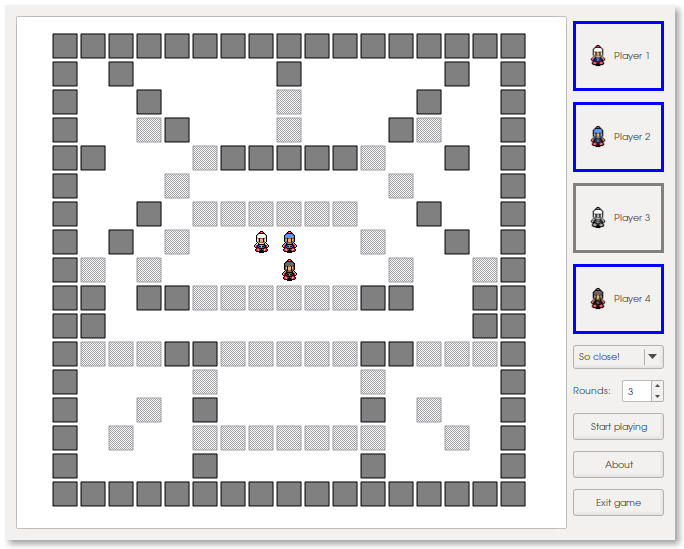
\includegraphics[width=\textwidth]{figures/qtalbomber.png}
  \caption{Unstarted game with three players}
\end{figure}

To activate or deactivate a player in the game, simply click on it icon
before starting the game. When the player icon borders are blue, the
player is active, when becoming red, the player is dead and gray border
means that the player is not active.
To distinguish players, refers to the player icon color.

\section{Application file architecture}

The \emph{Maps} directory contains the available game fields (see
map creation for more informations). Only maps in this directory will be
selected at game start.

The \emph{Sounds} directory includes sound files (\emph{.wav} format)
used by QtalBomber. If you want to change one or more of these sounds,
be sure to assign the filename that the one you are replacing.  Feel
free to add your favorite song as a soundtrack for your games!

\section{User controls}

\begin{center}
\begin{tabular}{l|c|c|c|c}
\toprule
Action      & Player 1           & Player 2 & Player 3 & Player 4 \\
\midrule
Up          & Top arrow          & Z        & U        & G        \\ 
Down        & Bottom arrow       & S        & J        & B        \\
Left        & Left arrow         & Q        & H        & V        \\
Right       & Right arrow        & D        & K        & N        \\
Drop bomb   & Cmd (or right Alt) & A        & Y        & Space    \\
\bottomrule
\end{tabular}
\end{center}



\section{Map creation}

You can create your own mazes game, use your imagination and creativity
to make maps new and fun. To do this, create an XML file according to
the maps available in the \emph{Maps} directory. See below for symbol
meaning and a map example.

\textbf{WARNING:} The card must not exceed 15x15 characters. The borders are generated
automatically, it is not necessary to draw them.  

\subsection{Available map symbols}

\begin{center}
\begin{tabular}{c | l}
\toprule
Symbol & Description \\
\midrule
\# & Unbreakable block \\
b & Breakable block \\
\_ & Unused space \\
1-4 & Start position of a player. Must be unique \\
\bottomrule
\end{tabular}
\end{center}

\subsection{Map XML example}

\lstinputlisting{../src/Maps/default.xml}

\end{document}
